%% recomposable_fragmentation.tex
%% Recomposable Fragmentation: A Field-Theoretic Critique of the Clip Economy
%% Flyxion (standardgalactic) — 2026

\documentclass{amsart}

%% ── Fonts & encoding ──────────────────────────────────────────────
\usepackage[T1]{fontenc}
\usepackage[utf8]{inputenc}
\usepackage{microtype}

%% ── Mathematics ───────────────────────────────────────────────────
\usepackage{amsmath,amssymb,amsthm}
\usepackage{mathtools}

%% ── Graphics & colour ─────────────────────────────────────────────
\usepackage{xcolor}
\usepackage{tikz}
\usetikzlibrary{arrows.meta, positioning, decorations.pathreplacing,
                shapes.geometric, fit, calc, backgrounds, matrix}

%% ── Layout ────────────────────────────────────────────────────────
\usepackage{geometry}
\geometry{margin=1.25in}
\usepackage{setspace}
\setstretch{1.08}

%% ── Tables ────────────────────────────────────────────────────────
\usepackage{booktabs}
\usepackage{array}

%% ── Hyperref ─────────────────────────────────────────────────────
\usepackage[
  colorlinks=true,
  linkcolor=darkblue,
  citecolor=darkblue,
  urlcolor=darkblue
]{hyperref}

%% ── Colours ───────────────────────────────────────────────────────
\definecolor{darkblue}{rgb}{0.08,0.20,0.45}
\definecolor{fieldgrey}{rgb}{0.92,0.92,0.94}
\definecolor{accentred}{rgb}{0.65,0.10,0.10}
\definecolor{structgreen}{rgb}{0.10,0.40,0.25}
\definecolor{warmgold}{rgb}{0.55,0.40,0.05}

%% ── Theorem environments ──────────────────────────────────────────
\theoremstyle{plain}
\newtheorem{theorem}{Theorem}[section]
\newtheorem{proposition}[theorem]{Proposition}
\newtheorem{lemma}[theorem]{Lemma}
\newtheorem{corollary}[theorem]{Corollary}

\theoremstyle{definition}
\newtheorem{definition}[theorem]{Definition}
\newtheorem{example}[theorem]{Example}
\newtheorem{construction}[theorem]{Construction}

\theoremstyle{remark}
\newtheorem{remark}[theorem]{Remark}
\newtheorem{observation}[theorem]{Observation}

%% ── Framed environments ───────────────────────────────────────────
\usepackage{mdframed}

\newmdenv[
  backgroundcolor=fieldgrey,
  linecolor=darkblue,
  linewidth=1.2pt,
  roundcorner=3pt,
  innertopmargin=7pt,
  innerbottommargin=7pt,
  skipabove=9pt,
  skipbelow=9pt
]{fieldbox}

\newmdenv[
  backgroundcolor=white,
  linecolor=accentred,
  linewidth=1.0pt,
  roundcorner=3pt,
  innertopmargin=6pt,
  innerbottommargin=6pt,
  skipabove=8pt,
  skipbelow=8pt
]{claimbox}

%% ── Macros ────────────────────────────────────────────────────────
\newcommand{\RSVP}{\textsc{rsvp}}
\newcommand{\scalar}{\Phi}
\newcommand{\vfield}{\mathbf{v}}
\newcommand{\entr}{S}
\newcommand{\vtrans}{\mathbf{v}_{\!\text{trans}}}
\newcommand{\vocc}{\mathbf{v}_{\!\text{occ}}}
\newcommand{\Man}{\mathcal{M}}
\newcommand{\Frag}{\mathcal{F}}
\newcommand{\Inj}{\mathcal{I}}
\newcommand{\Dec}{\mathcal{D}}
\newcommand{\Amp}{\mathcal{N}}
\newcommand{\Ectx}{\mathcal{E}}
\newcommand{\Rec}{\mathcal{R}}
\newcommand{\tensor}{\otimes}

%% ──────────────────────────────────────────────────────────────────
%% amsart uppercases the author in the running head via \MakeUppercase.
%% Redefining it to \@firstofone suppresses this globally, which is
%% safe here since section titles use \textsc, not \MakeUppercase.
\makeatletter
\let\MakeUppercase\@firstofone
\makeatother

\title[Recomposable Fragmentation]{%
  Recomposable Fragmentation:\\[4pt]
  \large A Field-Theoretic Critique of the Clip Economy
}

\author{Flyxion}
\address{Independent researcher, Canada}
\email{mechachleopteryx@gmail.com}
\date{April 2026}

\keywords{clip economy, recomposable fragmentation, semantic torsion,
          RSVP field theory, driven dissipative systems, admissible projection,
          Spherepop, trajectory-based cognition, occupation dynamics}

\subjclass[2020]{68T01, 91D30, 94A17, 37N99}

%% ──────────────────────────────────────────────────────────────────
\begin{document}

\begin{abstract}
The dominance of short-form media clips is not a cultural preference but a
structural phase transition in the physics of communication.  We model the clip
economy as a driven dissipative field system within the Relativistic
Scalar--Vector Plenum (\RSVP) framework, identifying engagement potential as a
scalar field $\scalar$, distributional flux as a vector field $\vfield$, and
context-loss as an entropy production term $\entr$.  The clip economy is not
merely turbulent; it is \emph{strategically overdriven}: the vector field
decomposes into a transport component $\vtrans$ and an occupation component
$\vocc$ that performs territorial saturation of the attentional manifold.
Coherence is not lost passively but is \emph{actively selected against}, since
compositional structure constitutes impedance drag in the transport layer.  We
sharpen the central diagnostic: the pathology is not fragmentation \emph{per se}
but \emph{non-recomposable} fragmentation---the production of units whose monoidal
composition yields no coherent global section.  Against this we define
\emph{admissible fragments}: units that are locally transmissible yet carry
explicit reconstruction data back to their origin manifold.  The system of all
such fragments, organised by a \emph{controlled projection layer} and governed by
an \emph{admissibility grammar}, constitutes an alternative field attractor
$(\scalar', \vfield', \entr')$ in which global compatibility is not erased by
transport.  We prove that this alternative is not merely philosophically preferable
but dynamically competitive: any coherence-preserving substrate must re-route the
existing energy flow rather than attempt to suppress it.
\end{abstract}

\maketitle
\newpage
\tableofcontents
\newpage

%% ══════════════════════════════════════════════════════════════════
\section{Introduction: A Phase Transition in Communication}
\label{sec:intro}
%% ══════════════════════════════════════════════════════════════════

Short-form media is not new.  The theatrical trailer, the newspaper headline, and
the radio spot have always co-existed with longer compositional forms.  What is
new---and what demands a structural rather than cultural account---is the inversion
of ontological priority: the clip has ceased to be a promotional teaser for a
longer work and has become the \emph{primary unit of consumption and monetisation}
in its own right.

This inversion is documented with precision in the economics of contemporary
streaming.  Platforms now sustain enormous apparent reach through clip circulation
entirely decoupled from the originating content.  A streamer may maintain a live
audience in the tens of thousands while generating billions of monthly views through
clips distributed by coordinated human and automated clipping operations.  The
``clipping army'' is not an external marketing layer; it is structural to the
content architecture.  Creators optimise their output so that any thirty-second
window is locally self-sufficient and algorithmically transmissible.  Legacy media
organisations are correspondingly advised to treat decades of archival footage not
as a library of finished works but as a \emph{reservoir of extractable moments}.

The standard cultural critique focuses on attention spans, reading rates, and
social isolation \cite{postman1985,han2015}.  These concerns may be warranted, but
they are empirically contested and theoretically imprecise.  The more tractable
claim is structural: the clip economy changes the \emph{unit of meaning}.  Long-form
content functioned as a semantic container in which coherence was internally
enforced---contradictions had to be resolved, arguments had to close, narratives had
to stabilise.  In the clip regime this enforcement is externalised to the algorithm,
which selects for local engagement without requiring global consistency
\cite{pariser2011,zeynep2015}.

The result is what we call \emph{semantic torsion}: a media field that is locally
smooth---every clip makes sense in the moment---but globally incompatible, in the
sense that the collection of clips circulating from any given source does not
compose into a recoverable whole.  The term is chosen deliberately: torsion in
differential geometry measures the failure of parallel transport to preserve
orientation \cite{munkres2000}.  A fragment understood at one point in the field,
and again at another, cannot be consistently embedded in a single global frame
without contradiction or amnesia.

This essay offers a formal account of these dynamics and derives from that account
a positive proposal: the system of \emph{admissible fragments}, organised by a
controlled projection layer and governed by an admissibility grammar, constitutes
an alternative attractor that is dynamically competitive rather than merely
philosophically preferable.

\begin{claimbox}
  \textbf{Central thesis.}  The pathology of the clip economy is not
  fragmentation but \emph{non-recomposable} fragmentation: the production of
  units optimised for terminal consumption rather than structured recombination.
  The alternative is not to restore long-form continuity but to enforce
  recomposability constraints on the fragment itself.
\end{claimbox}

The argument proceeds as follows.
Section~\ref{sec:field} introduces the field model.
Section~\ref{sec:overdriven} shows the system is strategically overdriven via the
occupation tensor.
Section~\ref{sec:atomic} proves the non-integrability of popularity in the atomic
limit.
Section~\ref{sec:torsion} analyses the phenomenological consequences.
Section~\ref{sec:recomposability} introduces the monoidal structure of
recomposable fragmentation.
Section~\ref{sec:failure} classifies the principal fragment failure modes.
Section~\ref{sec:admissible} defines admissible fragments formally.
Section~\ref{sec:grammar} formalises the admissibility grammar.
Section~\ref{sec:projection} describes the controlled projection layer.
Section~\ref{sec:topo-srs} develops topological spaced repetition and the
Spherepop substrate.
Section~\ref{sec:attractor} specifies the alternative attractor.
Section~\ref{sec:energetics} proves competitive viability.
Section~\ref{sec:conclusion} closes with the strategic reframing.

%% ══════════════════════════════════════════════════════════════════
\section{The Clip Economy as a Field System}
\label{sec:field}
%% ══════════════════════════════════════════════════════════════════

We model the clip economy through a coupled scalar--vector--entropy triple
$(\scalar, \vfield, \entr)$.  The framework is motivated by the treatment of
driven dissipative systems in \cite{cross1993,prigogine1984}: like those systems,
the clip economy maintains nonequilibrium structure through continuous energy
injection rather than settling to a thermal ground state.

\begin{definition}[Media field]
  \label{def:rsvp-media}
  Let $\Omega$ denote the attentional manifold: the space of possible positions in
  the distributional network.  The \emph{scalar engagement potential}
  $\scalar(u) \in \mathbb{R}_{\geq 0}$ measures the probability of momentary
  capture per unit exposure; in the clip regime $\scalar$ is not a measure of
  meaning or sustained attention but only the likelihood of a swipe-stop or click,
  and is maximised by units requiring zero prior context.  The \emph{vector
  distributional flux} $\vfield(u) \in T_u\Omega$ encodes the direction and
  magnitude of propagation through the network, supplied by algorithmic
  amplification and human clipping operations.  The \emph{entropy} $\entr(u)$
  measures the context-loss introduced by extracting $u$ from its source work, in
  the information-theoretic sense of \cite{shannon1948,cover2006}; high $\entr$
  correlates with high transmissibility because stripped context reduces the
  cognitive load required to consume the fragment.
\end{definition}

Let $\Inj(\vfield)$ denote the energy injected by clipping operations,
$\Dec(\scalar)$ the natural decay of engagement potential through attention fatigue,
$\Amp(\scalar)$ the nonlinear algorithmic amplification rewarding high-$\scalar$
fragments, $\Ectx(\scalar)$ the rate of context destruction per unit propagation,
and $\Rec$ the sparse global-synthesis attempts by individual consumers.  The field
dynamics are governed by the coupled system
\begin{align}
  \label{eq:phi-dynamics}
  \partial_t \scalar &= \Inj(\vfield) - \Dec(\scalar) + \Amp(\scalar), \\
  \label{eq:S-dynamics}
  \partial_t \entr   &= \Ectx(\scalar) - \Rec.
\end{align}
The key asymmetry captured by~\eqref{eq:S-dynamics} is that $\Ectx$ is large and
continuous---every act of clipping destroys some context, and by Landauer's
principle this erasure is thermodynamically irreversible \cite{landauer1961}---while
$\Rec$ is sparse and energetically costly.  Global sections therefore fail to form
not because they are impossible but because the rate of fragmentation structurally
exceeds the rate of recomposition.

\begin{proposition}
  \label{prop:entropy-advantage}
  In a field governed by~\eqref{eq:phi-dynamics}--\eqref{eq:S-dynamics}, entropy
  is a competitive advantage: stripping context from a unit $u$ increases
  $\scalar(u)$ by reducing the reconstruction burden on receivers, expanding the
  viable receiver population and increasing the magnitude of $\Amp(\scalar)$.
\end{proposition}

\begin{proof}[Sketch]
  Context encodes dependencies.  Dependencies impose reconstruction requirements
  that raise the effective cognitive load per unit \cite{kirschner2006}, reducing
  the population of receivers willing to engage.  A context-free fragment admits a
  maximal receiver population; under $\Amp$, monotone in the receiver population,
  this yields maximal $\partial_t \scalar$.
\end{proof}

The clip economy is therefore not malfunctioning.  It is a stable attractor under
a particular objective function.  Coherence is not lost through carelessness; it is
actively designed out of the production process to maximise flow through the
transport layer.

%% ══════════════════════════════════════════════════════════════════
\section{From Turbulence to Field Capture: The Occupation Tensor}
\label{sec:overdriven}
%% ══════════════════════════════════════════════════════════════════

A first-pass account treats the clip economy as semantically turbulent: local
vortices of engagement spin up and dissipate without coupling to a global
structure, in the pattern described by \cite{bak1996} for self-organised critical
systems.  This is correct but insufficient.  The more precise description is that
the system is \emph{strategically overdriven}: it does not merely distribute
high-$\scalar$ fragments, it actively suppresses competing signals by saturating
the available attentional bandwidth.

Coordinated clipping operations seed thousands of variants of the same content
across discovery algorithms.  The goal is not efficiency of transmission but
\emph{coverage}: the occupation of as many coordinates in clip-space as possible
\cite{barabasi2016,boyd2010}.  Creators and their agents monitor whether a given
coordinate is occupied; if it is not, it will be filled adversarially or
stochastically.  The implicit logic is territorial: if you are not there, they
will be.

\begin{definition}[Occupation tensor]
  \label{def:occupation}
  The distributional vector field decomposes as $\vfield = \vtrans + \vocc$, where
  $\vtrans$ is the \emph{transport component} moving a specific fragment from
  source to receiver, and $\vocc$ is the \emph{occupation component} filling
  attentional bandwidth to suppress competing signals.
\end{definition}

The occupation component introduces exclusion dynamics that have no analogue in
passive network diffusion models \cite{watts1998,newman2010}.  When $\|\vocc\|$ is
large, the background signal density rises until low-$\scalar$, high-coherence
content is filtered as noise.  The selection pressure is not merely \emph{for}
high-$\scalar$ fragments; it is actively \emph{against} the compositional structure
that would allow a global section to form.

\begin{proposition}
  \label{prop:coherence-drag}
  In a field with strong occupation dynamics, compositional structure functions as
  \emph{impedance drag}: a unit whose internal context requirements are high is
  mismatched to the transport layer and will be outcompeted by units with lower
  context requirements, even when the high-context unit carries greater semantic
  content.
\end{proposition}

Pre-emptive fragmentation---engineering content as a sequence of clip-ready spikes
rather than a continuous argument---is therefore an impedance-matching solution:
shaping $\scalar$ so that it survives advection under $\vfield$ while tolerating
high $\entr$.  In the language of Virilio's dromology \cite{virilio1986}, speed of
circulation has become the governing constraint, and coherence is precisely what
slows things down.

The financial energetics explain the system's stability.  The injection term
$\Inj(\vfield)$ is directly subsidised by economic incentives at scale: clipping
operations are funded as a line item, not a side effect.  The resulting
reinforcement forms a positive-feedback attractor \cite{strogatz2018}---clips
generate views and revenue, revenue funds further clipping, clipping increases
field occupation, and occupation increases the probability of viral
excitations---and because the system is externally subsidised, individual
withdrawal does not meaningfully reduce system energy.

\begin{center}
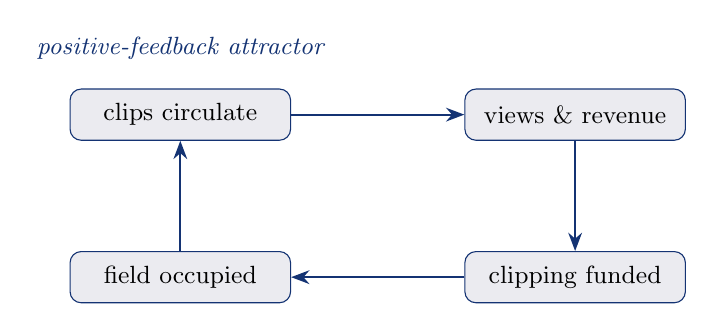
\begin{tikzpicture}[
  >=Stealth, node distance=1.4cm and 2.2cm,
  box/.style={draw=darkblue, rounded corners=4pt, fill=fieldgrey,
              minimum width=2.8cm, minimum height=0.65cm,
              font=\small, align=center},
  arr/.style={draw=darkblue, thick, ->}
]
  \node[box] (clips) {clips circulate};
  \node[box, right=of clips] (views) {views \& revenue};
  \node[box, below=of views] (funding) {clipping funded};
  \node[box, below=of clips] (occ) {field occupied};
  \draw[arr] (clips) -- (views);
  \draw[arr] (views) -- (funding);
  \draw[arr] (funding) -- (occ);
  \draw[arr] (occ) -- (clips);
  \node[font=\small\itshape, darkblue, above=0.25cm of clips]
    {positive-feedback attractor};
\end{tikzpicture}
\end{center}

%% ══════════════════════════════════════════════════════════════════
\section{The Atomic Limit and Non-Integrability of Popularity}
\label{sec:atomic}
%% ══════════════════════════════════════════════════════════════════

The clip economy admits a limiting case in which the fragment approaches a single
perceptual frame.  This limit clarifies the structural collapse of recomposability
and formalises the empirical observation that within the clip economy a view is a
view---popularity is treated as a purely additive quantity amenable to
straightforward aggregation, in the manner of a frequency count rather than a
measure on a structured space.

\begin{definition}[Atomic fragment]
  \label{def:atomic}
  An \emph{atomic fragment} is a fragment $f$ such that $\mathrm{supp}(f) \to 0$
  in both temporal and contextual extent while $\scalar(f)$ remains finite.
\end{definition}

In this limit, reconstruction becomes impossible by construction.  The fragment
contains no internal structure to support a recovery map $\rho_f$: there is no
source interval to cite, no prior argumentative state to reference, no dependency
graph to traverse.  The fragment is pure signal in the Shannon sense
\cite{shannon1948}---a symbol stripped of the pragmatic redundancy that would
allow error correction or source reconstruction.

\begin{proposition}[Non-integrability of popularity]
  \label{prop:nonintegrable}
  Let $\{f_i\}$ be a collection of atomic fragments generated from a source
  manifold $\Man$.  Then no finite measure $\mu$ on $\Frag$ exists such that
  \[
    \int_{\Frag} f_i \, d\mu \;\cong\; \Man.
  \]
\end{proposition}

\begin{proof}[Sketch]
  Atomic fragments erase ordering and dependency relations.  The integral reduces
  to a multiset of disjoint observations.  Since $\Man$ requires non-commutative
  composition (Definition~\ref{def:recomposable}), no measure preserving that
  structure exists: integration smears the very non-commutativity that encodes the
  source geometry \cite{lurie2009,maclane1998}.
\end{proof}

Popularity defined as aggregate view count is therefore constitutively blind to the
property that matters most for coherence preservation.  The integral diverges not
in the numerical sense but in the structural sense---the limit yields a flat
multiset rather than the curved manifold from which the fragments were extracted.
Any metric of success built on additive view aggregation cannot detect whether the
fragments it is counting are admissible or terminal.  The ``filter bubble''
described in \cite{pariser2011} is a downstream symptom of exactly this structural
blindness: a system optimised for additive engagement necessarily fails to track
whether the accumulated engagements compose into anything coherent.

%% ══════════════════════════════════════════════════════════════════
\section{Semantic Torsion and the Phenomenology of Global Failure}
\label{sec:torsion}
%% ══════════════════════════════════════════════════════════════════

The field analysis of Sections~\ref{sec:field}--\ref{sec:atomic} is external.  It
describes the mechanics of the clip economy from the perspective of an observer
mapping the field.  There is an internal dimension that the field equations alone
do not capture: the experience of inhabiting a system in which global coherence
never stabilises.

\begin{definition}[Semantic torsion]
  \label{def:torsion}
  A cognitive trajectory $\gamma\colon [0,T] \to \Man$ exhibits \emph{semantic
  torsion} if the parallel transport of local interpretive frames along $\gamma$
  fails to close: a fragment understood at time $t_1$ and again at time $t_2$ in a
  different distributional context cannot be embedded in a single consistent global
  frame without contradiction or amnesia.
\end{definition}

The term echoes holonomy in differential geometry \cite{munkres2000}: traversing a
loop in the field and returning to the starting point, one finds the frame has
rotated by an irreducible angle.  In the individual, this manifests as the
experience of encountering the same argument across different clip contexts and
finding that each encounter produces an incompatible local interpretation.

The transition from engagement to burnout to apathy traces a characteristic
trajectory in $\Man$.  Burnout is not a failure of effort; it is the accumulation
of semantic torsion beyond a recovery threshold.  In field terms, burnout
corresponds to a state of high $\scalar$, high $\|\vfield\|$, and unstable $\entr$:
the individual is still coupled to the flow but cannot integrate it.  Han's account
of the ``burnout society'' \cite{han2015} describes exactly this phenomenology at
the social scale---a culture that maximises performance output while destroying the
coherence structures that would make performance meaningful.  Apathy corresponds to
a collapse of coupling: the individual decouples from $\vfield$ entirely, achieving
local stability at the cost of forward-directed coherence.  Apathy is therefore not
the opposite of passion but its exhausted form, a distinction made structurally
precise by the Franklian observation \cite{frankl2006} that the loss of meaning is
not an affective event but a failure of the narrative trajectory that organises
action over time.

\begin{observation}
  Semantic torsion is not a pathology of individual attention capacity but a
  structural consequence of inhabiting a field with large $\|\vocc\|$ and minimal
  $\Rec$.  It is not addressable by exhortations to focus or curate but only by
  modifying the field structure or by providing the individual with an auxiliary
  manifold that supplies the missing global frame.
\end{observation}

The societal concern is therefore less about short attention spans in a simplistic
sense and more about the erosion of \emph{trajectory-based cognition}: the capacity
to hold unresolved structure over time, whether in reading, reasoning, or
relationships.  Kahneman's distinction between System 1 and System 2 cognition
\cite{kahneman2011} is relevant here not as a neural claim but as a structural one:
the clip economy continuously rewards fast, closure-seeking processing and
continuously fails to provide the conditions under which slow, structure-building
processing can operate.  If most inputs are fragments optimised for immediate
resolution, the cognitive practice of maintaining open structure as a condition of
eventual synthesis \cite{clark2013} becomes less exercised.  This does not imply
neurological damage, but it implies a shift in which cognitive skills are
reinforced by the ambient field.

%% ══════════════════════════════════════════════════════════════════
\section{Recomposability: The Structural Diagnosis}
\label{sec:recomposability}
%% ══════════════════════════════════════════════════════════════════

The analysis so far identifies what the clip economy destroys.  The central
diagnostic concept---the one that enables a positive proposal---is
\emph{recomposability}.  The pathology is not that fragments are short; it is that
they are non-recomposable.

\begin{definition}[Recomposable fragment system]
  \label{def:recomposable}
  A collection of fragments $\{u_i\}$ is \emph{recomposable} with respect to a
  source manifold $\Man$ if it satisfies three conditions.  \emph{Extraction
  validity} (R1): each $u_i$ retains meaning under extraction from $\Man$.
  \emph{Compositional gain} (R2): pairs $u_i \tensor u_j$ gain meaning---or at
  minimum do not lose meaning---under recombination.  \emph{Order sensitivity}
  (R3): the composition is non-commutative,
  \[
    u_i \tensor u_j \neq u_j \tensor u_i \quad \text{in general,}
  \]
  but both orderings remain meaningful, specifying a monoidal but non-symmetric
  structure \cite{maclane1998,baez2011}.
\end{definition}

Order sensitivity (R3) preserves the trajectory structure of an argument or
narrative: order matters without fully determining interpretation.  This is the
structure of jokes within a stand-up set, arguments within a conversation, and
ideas circulating across interviews.  Each of these evolved forms solved
recomposability before the algorithm needed to, developing modular units, repeatable
fragments, and flexible ordering while retaining narrative arc, speaker identity,
and thematic continuity \cite{boyd2010}.  The clip economy extracts the first
cluster of properties and discards the second.

\begin{proposition}
  \label{prop:nonrecomposable}
  The clip economy produces a degenerate fragment system satisfying~(R1) but
  violating~(R2) and~(R3).  Specifically, for typical clips $f_i, f_j$ drawn from
  the same source,
  \[
    f_i \tensor f_j \;\approx\; f_i \sqcup f_j,
  \]
  where $\sqcup$ denotes disjoint union: recombination yields juxtaposition
  without semantic gain, and the distinction between $f_i \tensor f_j$ and
  $f_j \tensor f_i$ is not structurally enforced.
\end{proposition}

This is the formal statement of semantic torsion at the algebraic level: locally
admissible fragments whose monoidal product fails to recover the source geometry.
Long-form media is not the opposite of clips; it is a \emph{disciplined
concatenation of recomposable clips under constraint}.  The failure of the current
ecosystem is that it discovered the unit but lost the discipline.

%% ══════════════════════════════════════════════════════════════════
\section{Failure Modes of Fragment Systems}
\label{sec:failure}
%% ══════════════════════════════════════════════════════════════════

To sharpen the admissibility condition it is useful to classify the principal ways
in which a fragment system can fail to be recomposable.  These failure modes
correspond directly to phenomena observable in the clip economy: decontextualised
quotation, ideological distortion, and algorithmically amplified misinterpretation
\cite{zeynep2015,doctorow2023}.

\begin{definition}[Terminal fragment]
  \label{def:terminal}
  A fragment $f$ is \emph{terminal} if its recovery map is empty,
  $\rho_f \equiv \varnothing$.  A terminal fragment resolves locally and admits no
  reconstruction path; it is designed to terminate traversal rather than trigger
  it.
\end{definition}

\begin{definition}[Drift fragment]
  \label{def:drift}
  A fragment $f$ exhibits \emph{semantic drift} if repeated transport under
  $\vfield$ deforms its recovery map, $\rho_f^{(t)} \not\cong \rho_f^{(0)}$.
  Each redistribution introduces a small perturbation to the implicit context in
  which $f$ is received, and these perturbations accumulate; after sufficient
  circulation, $f$ points to a manifold no longer isomorphic to the original
  source.  The mechanism is structurally analogous to the accumulation of
  measurement error under repeated resampling \cite{tversky1974}.
\end{definition}

\begin{definition}[Adversarial fragment]
  \label{def:adversarial}
  A fragment $f$ is \emph{adversarial} if its recovery map intentionally points to
  a manifold $\Man'$ not isomorphic to the original source $\Man$.  An adversarial
  fragment exploits local admissibility to route receivers toward a different global
  section than the one from which $f$ was ostensibly extracted.
\end{definition}

\begin{proposition}
  \label{prop:failure-modes}
  The clip economy maximises terminal fragments and tolerates drift and adversarial
  fragments as long as $\scalar$ is preserved.  The selection mechanism operates
  entirely on local engagement potential and is structurally blind to recovery map
  integrity.
\end{proposition}

The practical implication is that a high-$\scalar$ adversarial fragment is
indistinguishable from a high-$\scalar$ admissible fragment within the clip
economy's fitness function.  Any sufficiently coherent source manifold that
circulates via terminal or drift fragments will eventually be replaced, in the
attentional field, by adversarial reconstructions that it cannot correct from
within the same transport layer.  The strength of weak ties \cite{granovetter1973}
that would ordinarily diffuse adversarial content is here exploited by the
occupation component $\vocc$: the same bridging connections that spread information
across social clusters serve equally well to propagate adversarial recovery maps
without any mechanism to flag the distortion.

%% ══════════════════════════════════════════════════════════════════
\section{Admissible Fragments: A Formal Definition}
\label{sec:admissible}
%% ══════════════════════════════════════════════════════════════════

We now define the class of fragments that satisfy the recomposability conditions of
Definition~\ref{def:recomposable} while remaining transmissible in the existing
clip-economy transport layer.

\begin{definition}[Admissible fragment]
  \label{def:admissible}
  Let $\Man$ be the source manifold and let $\pi\colon \Man \to \Frag$ be a
  projection to a space of distributable fragments.  A fragment $f \in \Frag$ is
  \emph{admissible} if it satisfies three conditions simultaneously.
  \emph{Local transmissibility} (A1): $f$ is interpretable without reference to
  $\Man$ by a receiver with minimal background, achieving a viable $\scalar(f)$.
  \emph{Global recoverability} (A2): $f$ carries a recovery map
  $\rho_f\colon \Frag \dashrightarrow \Man$ such that $\rho_f(f)$ recovers the
  fibre $\pi^{-1}(f)$ up to a specified tolerance; concretely, $f$ encodes its
  source interval, prior argumentative context, subsequent context, speaker
  commitments, and known contradiction points.  \emph{Compositional compatibility}
  (A3): if $f_1, f_2$ are admissible fragments from the same region of $\Man$,
  then $\rho_{f_1}$ and $\rho_{f_2}$ extend to a common local section.  The
  admissibility condition is therefore:
  \[
    \text{fragment admissibility} =
    \text{local transmissibility} + \text{global recoverability}.
  \]
\end{definition}

Condition~(A1) is what the clip economy already delivers.  What it systematically
destroys are~(A2) and~(A3).  A clip's projection $\pi$ is \emph{degenerate}: it
maps many distinct regions of $\Man$ to a single high-$\scalar$ fragment, making
$\rho_f$ ill-defined \cite{spivak2014}.  An admissible fragment, by contrast,
functions as a \emph{partial chart} of the source manifold---small and locally
intelligible, yet carrying the transition maps needed to be glued to adjacent
charts, in precise analogy to the atlas construction in \cite{munkres2000}.

\begin{definition}[Holomorphic chart condition]
  \label{def:chart}
  An admissible fragment $f$ satisfies the \emph{holomorphic chart condition} if
  the recovery map $\rho_f$ is locally injective and its Jacobian preserves the
  orientation of the local section of $\Man$, so that the fragment not only points
  back to the source but does so in a way that respects the internal order structure
  of the argument.
\end{definition}

The crucial design inversion concerns tension.  A mainstream clip resolves tension
immediately because resolution maximises $\scalar$ by matching the fast-closure
preference of System 1 processing \cite{kahneman2011}.  An admissible fragment
must instead \emph{stabilise tension without resolving it}.  The signature of a
correctly constructed admissible fragment is the cognitive state: \textit{this
statement is precise, but I can see that it is not self-sufficient.}  This is
reconstruction pressure---a specific form of incompleteness creating motivation to
retrieve adjacent fragments without generating mere confusion.  In the predictive
processing framework of \cite{clark2013,friston2010}, it corresponds to a
calibrated prediction error: large enough to drive further sampling, small enough
not to trigger disengagement.

\begin{proposition}[Return probability]
  \label{prop:return}
  An admissible fragment $f$ generates a return probability
  \[
    p_{\mathrm{return}}(f, \sigma)
    = 1 - \exp\!\bigl(-\lambda\,|\partial f \setminus \sigma|\bigr),
  \]
  where $\sigma$ is the receiver's current covered region of $\Man$, $\partial f$
  is the set of fragments adjacent to $f$ in the source dependency graph, and
  $\lambda > 0$ measures the receiver's sensitivity to structural incompleteness.
  When $|\partial f \setminus \sigma|$ is large, $p_{\mathrm{return}} \to 1$: the
  fragment is an opening rather than a terminus.
\end{proposition}

Dense admissible fragments act as \emph{sinks} in the vector field $\vfield$,
drawing attention back toward the global section rather than releasing it into the
stream.  This is the structural analogue of the information foraging behaviour
described in \cite{pirolli1999}: a fragment with high ``information scent''---a
strong cue that valuable related content exists---produces greater dwell and
follow-through than one that exhausts its informational budget on first encounter.

%% ══════════════════════════════════════════════════════════════════
\section{The Admissibility Grammar}
\label{sec:grammar}
%% ══════════════════════════════════════════════════════════════════

The set of all admissible fragments is not merely a collection; it has the
structure of a generative system.  We formalise this as a grammar, emphasising
that the system's role is not archival---recording which fragments happen to satisfy
admissibility after the fact---but \emph{generative}: specifying the allowable
space of circulating units in advance.

\begin{definition}[Admissibility grammar]
  \label{def:grammar}
  An \emph{admissibility grammar} is a triple $\mathcal{G} = (\Sigma, R, \tau)$
  where $\Sigma$ is a set of primitive constraints on fragment form, $R$ is a set
  of composition rules specifying how admissible fragments may be combined, and
  $\tau$ assigns transition maps between adjacent fragments encoding their mutual
  reconstruction obligations.  A fragment $f$ is admissible in $\mathcal{G}$ if
  and only if it is derivable under $R$ from elements of $\Sigma$ and satisfies
  Definition~\ref{def:admissible}.
\end{definition}

The grammar $\mathcal{G}$ plays the role that the controlled projection layer plays
architecturally: it is the middle tier between the global theoretical system and
the circulating unit.  Where the clip economy has no such middle tier---fragments
are admitted or rejected by $\scalar$ alone---the grammar enforces structural
constraints on every emitted unit before it enters the field.  The formalism is
analogous to the typed calculi studied in \cite{baez2011}, in which morphisms carry
explicit information about their source and target objects.

\begin{theorem}[Closure under composition]
  \label{thm:closure}
  If $f_1$ and $f_2$ are admissible fragments generated by $\mathcal{G}$, then
  $f_1 \tensor f_2 \in \mathrm{Im}(\mathcal{G})$.
\end{theorem}

\begin{proof}
  Closure of $R$ under pairwise application ensures $f_1 \tensor f_2$ is
  derivable.  Compatibility of transition maps $\tau$ ensures that the composition
  inherits a recovery map pointing to the intersection of the fibres of $\rho_{f_1}$
  and $\rho_{f_2}$ in $\Man$, which is non-empty by condition~(A3) of
  Definition~\ref{def:admissible}.
\end{proof}

Theorem~\ref{thm:closure} means that the admissibility property is not fragile
under circulation: two admissible fragments composed by a receiver produce an
admissible result, not a terminal one.  The grammar is self-reinforcing; a field
populated primarily by admissible fragments will tend to remain so, because
compositions of admissible fragments are themselves admissible.

The grammar also makes precise the sense in which each unit should be written.  A
traditional proof is optimised for internal coherence, assuming a reader willing to
traverse the full argument \cite{lurie2009}.  An admissible proof has an additional
constraint: it must contain at least one \emph{projection-stable invariant}---a
statement that survives extraction and carries a trace of its dependencies.  Not a
slogan and not a summary, but a minimal fixed point of the argument.  Instead of
writing Constraint, then Local Result, then Proof, then Conclusion in a single
sealed unit, the admissible form writes Constraint, then Local Result, then
Boundary of Validity, then Pointer Outward---a structure that looks less like a
finished system and more like a field of stable partial structures, each of which
creates reconstruction pressure toward the next.

%% ══════════════════════════════════════════════════════════════════
\section{The Controlled Projection Layer}
\label{sec:projection}
%% ══════════════════════════════════════════════════════════════════

The design of admissible fragments requires a structural intermediate between the
global theoretical system and the circulating unit.  We call this the
\emph{controlled projection layer}.  Its existence is not hypothetical; it has been
discovered empirically, through practice, in high-density learning systems.

Consider the acquisition of a language through flashcard systems, or the
compression of a university course into Cornell-style cheat sheets.  These are
already clipping systems.  Each card or note is small, locally intelligible, and
rapidly transmissible.  Yet they behave entirely differently from the clip economy
because they preserve dependency structure.  A flashcard is not merely a fragment;
it is a fragment with an implicit reconstruction rule.  Encountering an Arabic
morphological pattern or a Spanish verb conjugation activates not a terminal
engagement event but a network of relations: grammar, phonology, prior exposures,
syntactic constraints.  The fragment is small; it is anchored to a latent structure.

\begin{example}[Flashcards as partial charts]
  \label{ex:flashcard}
  In a well-designed flashcard system \cite{wozniak1990,cepeda2006}, each card
  $(q, a)$ functions as a local chart of the knowledge manifold $\Man$: the
  question $q$ identifies a coordinate, the answer $a$ provides the local section,
  and the system's dependency graph encodes the transition maps between adjacent
  charts \cite{spivak2014}.  Learning the system amounts to internalising the
  atlas.  The learner does not need to hold the textbook in working memory; the
  textbook is reconstructed through the \emph{geometry of recall}.
\end{example}

The key distinction is directional rather than dimensional.  Atomisation does not
destroy coherence when each unit is a pointer into a latent network of relations.
What is required is that the network be explicitly designed and that units be
assigned positions within it.

The controlled projection layer is the middle tier of a three-tier structure
$\Man_0 \supset \Man_1 \supset \Man_2$, where containment is informational rather
than spatial.

\begin{definition}[Three-tier manifold]
  \label{def:three-tier}
  The \emph{global tier} $\Man_0$ is the fully articulated theoretical system---the
  textbook, formal treatise, or complete derivation---which defines the global
  geometry: all objects, all morphisms, all commutative diagrams \cite{maclane1998}.
  The \emph{structural tier} $\Man_1$ is the layer of structured compression: cheat
  sheets, conceptual maps, dependency graphs, preserving the relational skeleton of
  $\Man_0$ in compact form with objects retained and derivations compressed to
  transition maps.  The \emph{iterable tier} $\Man_2$ is the layer of circulating
  units---flashcards, clips, threads---each locally intelligible and each carrying
  a pointer into $\Man_1$.
\end{definition}

\begin{figure}[h]
\centering
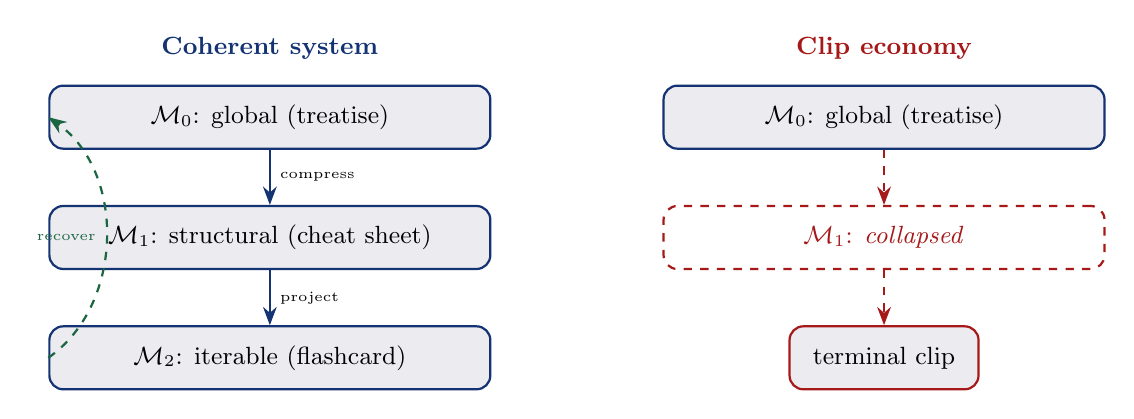
\begin{tikzpicture}[
  >=Stealth, node distance=0.7cm,
  tier/.style={draw=darkblue, thick, rounded corners=5pt,
               minimum width=5.6cm, minimum height=0.8cm,
               fill=fieldgrey, font=\small},
  dead/.style={draw=accentred, dashed, thick, rounded corners=5pt,
               minimum width=5.6cm, minimum height=0.8cm,
               font=\small, text=accentred},
  itm/.style={draw=accentred, thick, rounded corners=5pt,
              minimum width=2.4cm, minimum height=0.8cm,
              fill=fieldgrey, font=\small},
  arr/.style={draw=darkblue, thick, ->},
  rarr/.style={draw=structgreen, thick, dashed, ->}
]
  \node[tier] (M0) {$\Man_0$: global (treatise)};
  \node[tier, below=of M0] (M1) {$\Man_1$: structural (cheat sheet)};
  \node[tier, below=of M1] (M2) {$\Man_2$: iterable (flashcard)};
  \draw[arr] (M0) -- (M1) node[midway,right,font=\tiny] {compress};
  \draw[arr] (M1) -- (M2) node[midway,right,font=\tiny] {project};
  \draw[rarr, bend right=55] (M2.west)
    to node[left,font=\tiny,structgreen] {recover} (M0.west);
  \node[above=0.2cm of M0, font=\small\bfseries, darkblue] {Coherent system};
  \begin{scope}[xshift=7.8cm]
    \node[tier] (C0) {$\Man_0$: global (treatise)};
    \node[dead, below=of C0] (C1) {$\Man_1$: \emph{collapsed}};
    \node[itm, below=of C1] (C2) {terminal clip};
    \draw[draw=accentred, dashed, thick, ->] (C0) -- (C1);
    \draw[draw=accentred, dashed, thick, ->] (C1) -- (C2);
    \node[above=0.2cm of C0, font=\small\bfseries, accentred] {Clip economy};
  \end{scope}
\end{tikzpicture}
\caption{Left: the three-tier manifold, in which the structural tier $\Man_1$
provides recovery maps closing the loop from iterable units back to global theory.
Right: the clip economy collapses $\Man_1$, severing admissibility
conditions~(A2) and~(A3).  The controlled projection layer is precisely $\Man_1$.}
\label{fig:three-tier}
\end{figure}

The clip economy collapses $\Man_1$.  The global tier exists; the iterable tier
exists; the middle layer that would provide transition maps between them has been
eliminated.  Fragments at $\Man_2$ lose their pointers and remain locally
intelligible while the recovery map $\rho_f$ has no target structure to map into.
The result is what Postman diagnosed as the degradation of the ``typographic mind''
\cite{postman1985}, but what can now be specified more precisely: not a cultural
regression but the removal of the tier at which compositional constraints are
enforced.

%% ══════════════════════════════════════════════════════════════════
\section{Topological Spaced Repetition and the Spherepop Substrate}
\label{sec:topo-srs}
%% ══════════════════════════════════════════════════════════════════

The three-tier manifold suggests a reinterpretation of spaced repetition in
topological rather than temporal terms.  Standard systems such as Anki and SuperMemo
\cite{wozniak1990} schedule repetition by \emph{temporal decay}: items are
re-surfaced when recall probability falls below a threshold, treating forgetting as
the primary obstacle.  The empirical literature on distributed practice
\cite{cepeda2006} confirms the advantage of spaced over massed review, but the
scheduling principle remains temporal, independent of the geometric structure of
the knowledge manifold.

\begin{definition}[Coverage state]
  \label{def:coverage}
  Let $\sigma \subset \Man_1$ denote the learner's current covered region: the
  submanifold of the structural tier that the learner has successfully integrated
  into a locally consistent global section.
\end{definition}

\begin{definition}[Boundary scheduling]
  \label{def:boundary-sched}
  A fragment $f \in \Man_2$ is scheduled for re-presentation when
  $\partial f \cap (\Man_1 \setminus \sigma) \neq \varnothing$, that is, when at
  least one fragment adjacent to $f$ in the dependency graph has not yet been
  integrated into $\sigma$.
\end{definition}

\begin{proposition}
  \label{prop:topo-srs}
  Boundary scheduling minimises reconstruction error faster than temporal decay
  scheduling for any nontrivial dependency graph.
\end{proposition}

\begin{proof}[Sketch]
  Temporal scheduling ignores structural adjacency and may re-present items whose
  neighbours are already well-integrated---yielding redundant exposure---or defer
  items whose neighbours have an open boundary, missing the highest-information-gain
  opportunity.  Boundary scheduling targets exactly the edges of the dependency
  graph missing from $\sigma$, maximising expected semantic gain per unit of learner
  effort, in the sense made precise by information foraging theory \cite{pirolli1999}.
\end{proof}

Repetition is driven not by forgetting alone but by the geometry of the theory
being learned.  A fragment is re-presented not because time has elapsed but because
the learner's covered region has a specific gap that the fragment is positioned to
close.  Minimal guidance approaches \cite{kirschner2006} fail partly because they
provide no mechanism for tracking which gaps exist; boundary scheduling supplies
exactly this tracking.

The natural computational substrate for boundary scheduling is an irreversible-event
calculus in which each event consumes nested relational structure and leaves a
permanent trace, recording not merely what was encountered but in what order and
from which direction.  This allows the system to compute boundary membership---which
fragments lie on the frontier of $\sigma$---without maintaining a separate
forgetting model.  The learner's current state is not a snapshot but a trajectory,
and the set of available next events depends on the full sequence of prior events.
The thermodynamic irreversibility of each learning event is not incidental but
structural \cite{bennett1982,lloyd2000}: it is precisely because the events cannot
be undone that the trajectory they define has determinate content.

The dynamics of constraint accumulation in such a system connect to the field
description of Section~\ref{sec:field} through the following result.

\begin{theorem}[Field emergence from constraint accumulation]
  \label{thm:emergence}
  Let $\{C_n\}$ be a sequence of constraint accumulations in an irreversible-event
  system governed by the primitives of irreversibility, accumulation,
  compatibility, and flow.  As the lattice spacing $\epsilon \to 0$, the constraint
  density $\rho_n = |C_n|/\epsilon^d$ satisfies
  \[
    \partial_t \rho + \nabla \cdot (\rho\,\vfield) = \sigma,
  \]
  where $\vfield$ is the local constraint-propagation velocity and $\sigma$ is a
  source term corresponding to external inputs.  This is the scalar sector of the
  field equations of Section~\ref{sec:field}.
\end{theorem}

\begin{proof}[Sketch]
  The discrete accumulation satisfies a conservation law, since each event resolves
  exactly one open boundary segment.  Taylor expansion in $\epsilon$ yields the
  continuity equation, a standard coarse-graining argument in the spirit of
  \cite{cross1993,anderson1972}.  The identification of $\sigma$ with the scalar
  source follows from interpreting unresolved boundary as scalar field gradient.
\end{proof}

The learner therefore does not receive the field equations as axioms but discovers
them as the natural continuum analogue of the discrete constraint system already
internalised.  The more-is-different principle of \cite{anderson1972} applies: the
field description is not merely a rescaling of the discrete system but a genuinely
new level of description, with emergent phenomena not visible at the unit level.
The theory arrives as recognition rather than imposition.

%% ══════════════════════════════════════════════════════════════════
\section{The Alternative Attractor}
\label{sec:attractor}
%% ══════════════════════════════════════════════════════════════════

The foregoing analysis allows us to specify the alternative attractor precisely.
It is not ``restore long-form media'' and it is not ``reduce clips.''  It is a
field configuration $(\scalar', \vfield', \entr')$ satisfying three conditions
simultaneously: local admissibility remains high enough to propagate through the
existing transport layer, so $\scalar'(f) \geq \scalar_{\min}$ for all circulating
fragments; global compatibility is not erased by transport, so the composition
$f_i \tensor f_j$ recovers a section of $\Man_1$ for all admissible pairs; and the
entropy production rate is bounded, $\partial_t \entr' \leq \kappa$, for some
constant $\kappa$ determined by the reconstruction capacity $\Rec$.

The alternative attractor is not a retreat from the clip layer but a re-routing of
the existing flow through a manifold that enforces constraint closure
\cite{prigogine1984,strogatz2018}.  The clipping army, understood as a distributed
pump, is not dismantled; its output is redirected through fragments that carry
their own reconstruction data.

The producer operating under this constraint is not producing clips or textbooks.
They are defining a \emph{strategic functor}
\[
  \mathcal{F}\colon \text{Coherent System} \to \text{Fragment Space}
\]
with the property that every fragment carries a left-inverse---or at minimum a
homotopy back---to its source \cite{maclane1998,spivak2014}.  The clip economy
uses a degenerate version,
$\mathcal{F}_{\text{clip}}\colon \text{Anything} \to \text{High-}\scalar\text{
fragment}$,
with no inverse, no structure preservation, and no obligation to recombine.  The
correct strategic sequence is therefore:
\begin{equation}
  \label{eq:strategic-sequence}
  \text{Coherent Work}
  \;\xrightarrow{\;\text{define}\;}\;
  \text{Controlled Projection Layer}
  \;\xrightarrow{\;\text{emit}\;}\;
  \text{Field Circulation.}
\end{equation}

Without the middle step, the projection happens anyway---but without the producer's
constraints.  The coherent system becomes raw material for the very fragmentation
it was designed to resist, as Debord's analysis of the spectacle anticipates
\cite{debord1967}: the image circulates freely precisely because it has been
severed from the conditions of its production.  The alternative scaling strategy is
therefore not volume~$\to$~saturation but \emph{consistency~$\to$~accumulation}:
the same admissible fragments appear across different contexts, gradually building
a coherent basin of attraction through the weak-tie diffusion described in
\cite{granovetter1973}, but now channelled through admissible recovery maps rather
than terminal projections.

%% ══════════════════════════════════════════════════════════════════
\section{Energetic Competition and Field Stability}
\label{sec:energetics}
%% ══════════════════════════════════════════════════════════════════

The alternative attractor must be not only formally coherent but energetically
viable.  Any coherence-preserving system that cannot sustain injection comparable
to the clip economy will be overwhelmed by the existing flow rather than competing
with it \cite{cross1993,strogatz2018}.

\begin{definition}[Field stability]
  \label{def:stability}
  An attractor $(\scalar', \vfield', \entr')$ is \emph{dynamically stable} if
  \[
    \frac{d}{dt} \int_{\Omega} \scalar' \, d\Omega \;\geq\; 0
  \]
  under perturbations induced by the clip economy field, maintaining or increasing
  its total engagement potential against the competing flow.
\end{definition}

\begin{theorem}[Competitive viability]
  \label{thm:viability}
  An admissible fragment system is dynamically stable if and only if
  \[
    \Inj(\vfield') \;\geq\; \Inj(\vfield_{\text{clip}}) - \epsilon
  \]
  for some bounded $\epsilon > 0$.
\end{theorem}

\begin{proof}[Sketch]
  If injection falls below the competing field by more than $\epsilon$, the
  occupation dynamics of $\vocc$ dominate: background signal density rises until
  high-coherence units are filtered as noise and the admissible fragment system
  collapses into terminal fragmentation.  Conversely, if injection is within
  $\epsilon$ of the competing field, the return-probability mechanism of
  Proposition~\ref{prop:return} produces a self-sustaining basin: each admissible
  fragment draws receivers back, supplying a secondary injection channel that
  compensates for any deficit in the primary flow.  The argument follows the
  basin-of-attraction analysis in \cite{strogatz2018}, applied to the
  two-attractor competition between $\vfield$ and $\vfield'$.
\end{proof}

Theorem~\ref{thm:viability} makes precise why coherence-preserving systems must
re-route the existing flow rather than reject it.  A system that refuses to
participate in the clip layer---no matter how formally coherent---will be outcompeted
by the occupation dynamics of $\vocc$ and become invisible in the attentional
field.  The upper bound on computational and physical resources available to any
information-processing system \cite{lloyd2000} applies here as well: there is a
finite attentional budget, and a system that does not compete for it cedes it
entirely.

This also clarifies the relationship between a textbook-first production strategy
and the controlled projection layer.  Building the global tier $\Man_0$ first is
accumulation of potential energy; when projection eventually occurs, the density of
the admissible fragments is sufficient to create field sinks that the clip economy
cannot produce---units that reward deeper traversal, create recurring curvature in
the field rather than one-time spikes, and gradually build a coherent basin of
attraction through consistency rather than through volume.  These are genuinely
different attractors, and Theorem~\ref{thm:viability} identifies the minimum
injection condition that separates them.

%% ══════════════════════════════════════════════════════════════════
\section{Conclusion: Fragments That Cannot Be Fully Consumed}
\label{sec:conclusion}
%% ══════════════════════════════════════════════════════════════════

The clip economy discovered the unit but lost the discipline.  It solved the
problem of transmissibility at the cost of recomposability.  The result is a media
environment in which meaning is local, popularity is non-integrable, and
trajectory-based cognition is systematically under-rewarded.

The framework developed in this essay constitutes a complete formal system.  At
the ontological level, the field triple $(\scalar, \vfield, \entr)$ models the
clip economy as a driven dissipative system with occupation dynamics
\cite{cross1993,prigogine1984}.  At the algebraic level, the monoidal structure of
Definition~\ref{def:recomposable} distinguishes recomposable from non-recomposable
fragmentation \cite{maclane1998,baez2011}.  At the logical level, the admissibility
grammar $\mathcal{G}$ generates the allowable space of circulating units and closes
under composition (Theorem~\ref{thm:closure}).  At the dynamical level, the field
stability theorem (Theorem~\ref{thm:viability}) proves the minimum injection
condition for competitive viability \cite{strogatz2018}.  At the computational
level, the irreversible-event substrate and topological spaced repetition supply
the mechanism for constraint accumulation and boundary-driven scheduling
\cite{bennett1982,lloyd2000}, and the field equations emerge from that substrate in
the continuum limit (Theorem~\ref{thm:emergence}) \cite{anderson1972,cross1993}.

\begin{claimbox}
  \textbf{Final formulation.}  Long-form media is not the opposite of clips.  It
  is a disciplined concatenation of recomposable clips under constraint.  The
  failure of the current ecosystem is that it discovered the unit but lost the
  discipline.  The project of recomposable fragmentation is to restore that
  discipline in a form that can survive modern transport---not by refusing the
  field, but by introducing into it a different geometry.
\end{claimbox}

This requires defining a new class of object: a fragment that cannot be fully
consumed without becoming something else---either expanded, revisited, or
recontextualised.  Such a fragment is fundamentally incompatible with the clip
economy's dependence on terminal consumption, yet compatible with the transport
layer because it achieves a viable $\scalar(f)$.  It does not refuse the field; it
introduces a different geometry into it.

The unit of meaning, on this account, is not the clip, the article, or the theory
itself, but the \emph{trajectory of constraint integration} that unfolds over time
in a mind that has encountered enough admissible fragments to triangulate the source
manifold.  What the controlled projection layer produces is not knowledge
transferred but knowledge made recoverable: the conditions under which a coherent
structure can be reconstructed within the minds of its participants, even when
those participants encounter it one admissible fragment at a time.

\newpage
%% ══════════════════════════════════════════════════════════════════
\begin{thebibliography}{99}

\bibitem{maclane1998}
  S.\ Mac Lane,
  \textit{Categories for the Working Mathematician},
  2nd ed., Springer, New York, 1998.

\bibitem{baez2011}
  J.\ C.\ Baez and J.\ P.\ Stay,
  Physics, topology, logic and computation: a Rosetta Stone,
  \textit{New Structures for Physics}, Lecture Notes in Physics 813,
  Springer, 2011, 95--172.

\bibitem{lurie2009}
  J.\ Lurie,
  \textit{Higher Topos Theory},
  Princeton University Press, Princeton, 2009.

\bibitem{munkres2000}
  J.\ R.\ Munkres,
  \textit{Topology},
  2nd ed., Prentice Hall, Upper Saddle River, 2000.

\bibitem{spivak2014}
  D.\ I.\ Spivak,
  \textit{Category Theory for the Sciences},
  MIT Press, Cambridge, 2014.

\bibitem{shannon1948}
  C.\ E.\ Shannon,
  A mathematical theory of communication,
  \textit{Bell System Technical Journal} \textbf{27} (1948), 379--423, 623--656.

\bibitem{cover2006}
  T.\ M.\ Cover and J.\ A.\ Thomas,
  \textit{Elements of Information Theory},
  2nd ed., Wiley, 2006.

\bibitem{landauer1961}
  R.\ Landauer,
  Irreversibility and heat generation in the computing process,
  \textit{IBM Journal of Research and Development} \textbf{5} (1961), 183--191.

\bibitem{bennett1982}
  C.\ H.\ Bennett,
  The thermodynamics of computation,
  \textit{International Journal of Theoretical Physics} \textbf{21} (1982), 905--940.

\bibitem{lloyd2000}
  S.\ Lloyd,
  Ultimate physical limits to computation,
  \textit{Nature} \textbf{406} (2000), 1047--1054.

\bibitem{cross1993}
  M.\ C.\ Cross and P.\ C.\ Hohenberg,
  Pattern formation outside of equilibrium,
  \textit{Rev.\ Mod.\ Phys.}\ \textbf{65} (1993), 851--1112.

\bibitem{strogatz2018}
  S.\ H.\ Strogatz,
  \textit{Nonlinear Dynamics and Chaos},
  2nd ed., Westview Press, 2018.

\bibitem{prigogine1984}
  I.\ Prigogine and I.\ Stengers,
  \textit{Order Out of Chaos},
  Bantam Books, 1984.

\bibitem{bak1996}
  P.\ Bak,
  \textit{How Nature Works: The Science of Self-Organized Criticality},
  Springer, 1996.

\bibitem{anderson1972}
  P.\ W.\ Anderson,
  More is different,
  \textit{Science} \textbf{177} (1972), 393--396.

\bibitem{kahneman2011}
  D.\ Kahneman,
  \textit{Thinking, Fast and Slow},
  Farrar, Straus and Giroux, 2011.

\bibitem{tversky1974}
  A.\ Tversky and D.\ Kahneman,
  Judgment under uncertainty: heuristics and biases,
  \textit{Science} \textbf{185} (1974), 1124--1131.

\bibitem{clark2013}
  A.\ Clark,
  \textit{Surfing Uncertainty: Prediction, Action, and the Embodied Mind},
  Oxford University Press, 2013.

\bibitem{friston2010}
  K.\ Friston,
  The free-energy principle: a unified brain theory?,
  \textit{Nature Reviews Neuroscience} \textbf{11} (2010), 127--138.

\bibitem{pirolli1999}
  P.\ Pirolli and S.\ Card,
  Information foraging,
  \textit{Psychological Review} \textbf{106} (1999), 643--675.

\bibitem{wozniak1990}
  P.\ Wo\'zniak,
  \textit{SuperMemo: The Fastest and Most Effective Method of Learning},
  SuperMemo World, 1990.

\bibitem{cepeda2006}
  N.\ J.\ Cepeda et al.,
  Distributed practice in verbal recall tasks,
  \textit{Psychological Bulletin} \textbf{132} (2006), 354--380.

\bibitem{kirschner2006}
  P.\ A.\ Kirschner, J.\ Sweller, and R.\ E.\ Clark,
  Why minimal guidance during instruction does not work,
  \textit{Educational Psychologist} \textbf{41} (2006), 75--86.

\bibitem{postman1985}
  N.\ Postman,
  \textit{Amusing Ourselves to Death},
  Penguin Books, 1985.

\bibitem{debord1967}
  G.\ Debord,
  \textit{The Society of the Spectacle},
  Black \& Red, 1967.

\bibitem{virilio1986}
  P.\ Virilio,
  \textit{Speed and Politics},
  Semiotext(e), 1986.

\bibitem{han2015}
  B.-C.\ Han,
  \textit{The Burnout Society},
  Stanford University Press, 2015.

\bibitem{doctorow2023}
  C.\ Doctorow,
  Tiktok's enshittification,
  \textit{Pluralistic}, January 2023,
  \url{https://pluralistic.net/2023/01/21/potemkin-ai/}.

\bibitem{zeynep2015}
  Z.\ Tufekci,
  Algorithmic harms beyond Facebook and Google,
  \textit{Colorado Technology Law Journal} \textbf{13} (2015), 203--218.

\bibitem{pariser2011}
  E.\ Pariser,
  \textit{The Filter Bubble},
  Penguin Press, 2011.

\bibitem{boyd2010}
  d.\ boyd,
  Social network sites as networked publics,
  \textit{A Networked Self}, Routledge, 2010.

\bibitem{barabasi2016}
  A.-L.\ Barab\'asi,
  \textit{Network Science},
  Cambridge University Press, 2016.

\bibitem{newman2010}
  M.\ E.\ J.\ Newman,
  \textit{Networks: An Introduction},
  Oxford University Press, 2010.

\bibitem{watts1998}
  D.\ J.\ Watts and S.\ H.\ Strogatz,
  Collective dynamics of small-world networks,
  \textit{Nature} \textbf{393} (1998), 440--442.

\bibitem{granovetter1973}
  M.\ Granovetter,
  The strength of weak ties,
  \textit{American Journal of Sociology} \textbf{78} (1973), 1360--1380.

\bibitem{frankl2006}
  V.\ E.\ Frankl,
  \textit{Man's Search for Meaning},
  Beacon Press, Boston, 2006.

\end{thebibliography}
%% ══════════════════════════════════════════════════════════════════

\end{document}
